\section{Implementación de Atractor Determinístico - Estocástico}
\label{sec:AnalysisImpLorenz}

En aplicaciones digitales, el tiempo y la variable de estado tienen valores discretos.
La discretización de tiempo impone el uso de un algoritmo para aproximar las ecuaciones diferenciales de tiempo continuo que modelan el sistema.
El algoritmo más simple es el método de Euler de primer orden en el que los diferenciales se reemplazan directamente por incrementos finitos.
Los algoritmos más elaborados, como los algoritmos de paso variable Runge-Kutta de cuarto orden (RK4) (o superior), hacen que el sistema discreto evolucione más cerca del sistema continuo, pero con mayores requisitos de recursos de hardware y tiempos de cálculo.
En consecuencia, deben usarse solo si la exactitud es un requisito de la aplicación específica.
Este no es el caso en PRNG, donde la aleatoriedad es la característica principal que debe garantizarse.

Como se dijo anteriormente la cantidad de bits a emplearse es un tema crítico en la implementación de sistemas caóticos. Se han propuesto varias estrategias para una selección correcta del número óptimo de bits en las implementaciones en hardware.
Sin embargo, la mayoría de estos procedimientos están limitados a sistemas lineales \cite{Constantinides2002, Constantinides2003}.
En los sistemas digitales caóticos, se puede obtener un comportamiento completamente diferente al variar la precisión.
Este problema ha ganado interés recientemente, y se han propuesto varios esquemas nuevos \cite{Ding2007, Asseri2002, Azzaz2009}.

En resumen, a pesar de la aritmética utilizada, ya sea de punto fijo o punto flotante, el conjunto de números que se pueden representar es limitado.
Incluso utilizando una precisión extremadamente alta como lo hacen Liao y Wang \cite{Liao2013a}, las secuencias generadas por un sistema caótico que usa hardware digital siempre serán periódicas.

En esta Sección, se implementó un oscilador discreto de Lorenz obtenido mediante el uso del algoritmo de primer orden de Euler y tres estándares de representación diferentes.
Además se aplicaron técnicas de aleatorización a las variables de estado para obtener un PRNG en tiempo real.
El objetivo de este trabajo es estudiar la influencia del procedimiento de discretización en la dinámica del sistema.
En \cite{DeMicco2010} se estudió el grado de estocasticidad de un sistema caótico determinista mediante su implementación en coma flotante de precisión simple (32 bits estándar IEEE 754).

Se eligió el sistema caótico de Lorenz porque es un sistema ampliamente estudiado y también ha sido implementado por otros autores con diferentes metodologías \cite{Asseri2002, Azzaz2009, Azzaz2010}.
Por ejemplo, en \cite{Asseri2002}, se implementó un oscilador caótico de Lorenz mediante una toolbox del Generador de Sistemas Xilinx que funciona bajo MATLAB-Simulink.
Esta toolbox convierte el modelo MATLAB-Simulink en el modelo de Xilinx System Generator y luego se obtiene el código VHDL.
Esta herramienta, si bien facilita la implementación, al realizar una operación automática no permite ciertos cambios específicos y presenta algunas limitaciones.
La operación de integración se aproximó con el algoritmo de Euler, utilizando bloques de suma y retardo.
La implementación propuesta en \cite{Azzaz2009} y \cite{Azzaz2010} usa RK4 en una arquitectura de punto fijo de $32$ bits.

Se utilizó el software QuartusII 7.2 para generar el lenguaje de descripción de hardware VHDL y la implementación física se realizó en la placa de desarrollo Altera Cyclone III EP3C12.
Se estudiaron tres representaciones numéricas:
1) punto flotante estándar IEEE 754,
2) punto fijo decimal, y
3) aritmética entera \cite{Gonzalez2003}.
Cada representación implica una cantidad diferente de bits.
Consideramos dos representaciones de coma flotante para los estándares simple o doble, con $32$ y $64$ bits respectivamente para representar el signo, el exponente y la mantisa.
La aritmética decimal de punto fijo usa $p$ bits para representar la parte entera y $m$ bits para representar la parte fraccional.
Se consideraron representaciones de punto fijo de $32$ y $64$ bits con $9$ bits para la parte entera y $1$ bit para el signo y los $22$ o $54$ bits restantes para la parte fraccionaria.
En aritmética de enteros $k$ bits el alfabeto tiene $2^k$ símbolos.
Consideramos $k=54$.

Para cuantificar la aleatoriedad del sistema, se utilizó el conjunto de pruebas DIEHARD de Marsaglia \cite{Marsaglia1995}.
Estas pruebas han sido ampliamente utilizadas en la literatura abierta y son muy efectivas para clasificar sistemas determinísticos y estocásticos.

\subsection{Discretización Temporal del Oscilador de Lorenz}
\label{sec:lorenzdigit}

El sistema de Lorenz se define mediante el siguiente conjunto de ecuaciones diferenciales ordinarias acopladas:
%
\begin{eqnarray} \label{eq:lorconti}
\frac{dx}{dt}&=&-\delta(x-y) \ , \nonumber \\
\frac{dy}{dt}&=&\Gamma x-y-xz \ , \\
\frac{dz}{dt}&=&-bz+xy \ , \nonumber
\end{eqnarray}
%
donde $\delta$, $\Gamma$ y $b$ son parámetros constructivos del sistema.
Para ciertos valores de estos parámetros, el sistema tiene un comportamiento caótico.
Para convertir un sistema dinámico continuo en un sistema dinámico de tiempo discreto se requiere emplear algún algoritmo.
El algoritmo más simple fue propuesto por Euler y, para las Ecuaciones \ref{eq:lorconti} surge el siguiente modelo discreto:
%
\begin{eqnarray}\label{eq:loreuler}
{\widetilde X}_{t+\Delta t}&=&{\widetilde X}_{t}+ \Delta t \left[
- \delta \left( {\widetilde X}_{t}-{\widetilde Y}_{t} \right)
\right]
\ , \nonumber \\
{\widetilde Y}_{t+\Delta t}&=&{\widetilde Y}_{t}+ \Delta t \left[
-{\widetilde X}_{t}{\widetilde Z}_{t}+\Gamma~{\widetilde
X}_{t}-{\widetilde Y}_{t} \right] \ ,
\\
{\widetilde Z}_{t+\Delta t}&=&{\widetilde Z}_{t}+ \Delta t \left[
{\widetilde X}_{t}{\widetilde Y}_{t}-b~{\widetilde Z}_{t} \right]
\ , \nonumber
\end{eqnarray}
%
donde $\Delta t$ es el tamaño de paso de tiempo y $\widetilde X$, $\widetilde Y$ y $\widetilde Z$ son variables de estado de tiempo discreto que toman valores reales.

El algoritmo de Euler es un algoritmo de un sólo paso porque para calcular las variables en el momento $t + \Delta t$, sólo es necesario conocer los valores en el instante anterior.
Calculando iterativamente con un paso $\Delta t$ apropiado, es posible obtener la evolución del sistema discreto.
Es razonable esperar que cuanto menor sea el valor de $\Delta t$, más exactos serán los valores obtenidos.
Sin embargo, se debe tener en cuenta que al reducir el valor de $\Delta t$ se incrementa la cantidad de cálculos y esto genera más errores de redondeo.

En aplicaciones que requieren una reproducción exacta de la dinámica del sistema continuo, los algoritmos más exactos son obligatorios, pero en el caso de los PRNG, solo las propiedades estadísticas y la aleatoriedad de las series temporales son importantes y, por consiguiente, en este caso el algoritmo de Euler es lo suficientemente bueno.

\subsection{Discretización de las Variables de Estado}
\label{sec:numrepre}

Como se señaló anteriormente, se utilizan tres representaciones numéricas diferentes.
Cada una se describe en las siguientes Subsecciones.

\subsubsection{Estándar IEEE 754}
\label{sec:impleFloat}

La representación en punto flotante es uno de los métodos para representar números reales con precisión finita.
La ventaja de la representación de punto flotante sobre las representaciones de punto fijo y entero es que puede admitir un rango de valores mucho más amplio porque escala automáticamente cada número para usar la longitud de palabra completa para la mantisa; esto se hace moviendo el punto decimal (este procedimiento implica un cambio en el valor del exponente) hacia la posición del bit más significativo.
En consecuencia, la precisión total se conserva incluso para números pequeños.
La aritmética de punto flotante binaria es más adecuada para trabajar con cantidades del mundo real en una amplia gama de escalas.

El estándar de precisión simple IEEE 754 asigna $23$ bits a la mantisa (bit $0$ a $22$), el exponente ocupa los siguientes $8$ bits ($23$ a $30$) y el bit $31$ está asignado al signo.
El estándar de precisión doble IEEE 754 asigna $52$ bits a la mantisa (bit $0$ a $51$), el exponente ocupa los siguientes $11$ bits ($52$ a $62$) y el bit $63$ está asignado al signo.

Las operaciones aritméticas de punto flotante son más complicadas que las de punto fijo.
Su ejecución requiere más ciclos de reloj y hardware complejo.
Sin embargo, gracias al avance tecnológico y al desarrollo de nuevos materiales, la cantidad de recursos, memoria y frecuencia de operación de los dispositivos digitales se incrementa constantemente.
Hoy en día existen FPGAs con más memoria y recursos, capaces de trabajar a altas frecuencias en estos estándares.

\subsubsection{Implementación en Punto Fijo}
\label{sec:impleFix}

Cuando todos los valores a utilizar se encuentran dentro de un rango conocido, es posible lograr una mayor precisión utilizando la denominada representación de punto fijo en lugar de la representación de punto flotante.
El hardware requerido para manipular estas representaciones es el mismo comúnmente utilizado para realizar operaciones enteras y es menos costoso que el requerido para el caso de punto flotante.

Para evitar el desbordamiento, inicialmente es necesario realizar un análisis para determinar los valores extremos involucrados en el cálculo, incluidas las operaciones intermedias.
Con esta información, se determina el número mínimo de bits que se emplearán.
Una vez establecido el número de bits necesarios para representar la parte entera, se usa un bit adicional para representar números negativos basados en complemanto a 2 (CA2).
Los bits restantes se utilizan para mejorar la precisión ya que representan la parte fraccionaria.

Las operaciones de suma, resta y multiplicación se implementan de la misma manera que en la aritmética de enteros.
Solo es necesario cuidar la posición del punto que separa la parte entera de la fraccionaria.

Aquí consideramos dos casos, $32$ y $64$ bits por cada número entero.
En ambos casos se usaron $9$ bits para la parte entera, más $1$ bit para el signo, dejando los bits restantes, $22$ o $54$ respectivamente, para la parte decimal.

\subsubsection{Impelmentación en Aritmética Entera}
\label{sec:impleInt}

En aritmética de enteros, los circuitos se pueden reducir significativamente si se adoptan divisores con una potencia de $2$.
Para obtener la versión entera para el sistema Lorenz, se realizaron las siguientes transformaciones de polarización y escalado.
La polarización consiste en un corrimiento respecto de los ejes coordenados y el escalado en una contracción o expansión de estos ejes \cite{Gonzalez2003}:
%
\begin{eqnarray} \label{eq:newvariables}
{X}_{t}&=&\left({\widetilde X}_{t} + B\right)S \ , \nonumber \\
{Y}_{t}&=&\left({\widetilde Y}_{t} + B\right)S \ , \\
{Z}_{t}&=&\left({\widetilde Z}_{t} + B\right)S \ , \nonumber
\end{eqnarray}
%
donde $ B $ y $ S $ son los parámetros de polarización y escala, respectivamente.
Reemplazando la Ecuación \ref {eq:newvariables} en \ref{eq:loreuler} se obtiene:
%
\begin{eqnarray}\label{eq:Lorenz2}
{X}_{t+\Delta t}&=& {X}_{t} + \Delta t \ \delta~\left( {Y}_{t} -
{X}_{t} \right)
\ ,\nonumber \\
{Y}_{t+\Delta t}&=&(1- \Delta t )~{Y}_{t}+ \Delta t \
(B+\Gamma)~{X}_{t}~+~
\Delta t ~B~{Z}_{t} \nonumber\\
&~&-{\frac{\Delta t}{S}}{X}_{t}{Z}_{t}+ \Delta t \ BS(1-\Gamma-B) \ ,\\
{Z}_{t+\Delta t}&=&(1-\Delta t b){Z}_{t}-\Delta t B\left( {X}_{t}
+
{Y}_{t} \right)\nonumber \\
&&+{\frac{\Delta t}{S}}{X}_{t}{Y}_{t}+ \Delta t \ BS(B-b) \ .
\nonumber
\end{eqnarray}
%
En este caso, fue adoptado: $\delta=8$, $\Gamma=24$, $b=2$, $\Delta t \ =2^{-n}$, $B=40$, $S=512$. La variable $n$ es un número entero que dejamos libre para poder explorar el comportamiento del sistema con distintos pasos de tiempo.

Debe tenerse cuidado cuando se eligen los parámetros del sistema, en este caso se seleccionaron coeficientes enteros y se realizó un análisis de estabilidad para garantizar que el sistema no converja a un punto fijo o a una órbita de período bajo.

El sistema final es:
%
\begin{eqnarray}\label{eq:Lorenz3}
{X}_{t+\Delta t}&=&{X}_{t}+floor\left[ {\frac{{Y}_{t}}{2^{{n-3}}}}
\right] -floor\left[{\frac{{X}_{t}}{2^{{n-3}}}}\right] \ , \nonumber \\
{Y}_{t+\Delta t}&=&{Y}_{t}-floor\left[
{\frac{{Y}_{t}}{2^n}}\right]
+floor\left[{\frac{{X}_{t}}{2^{{n-6}}}}\right]\nonumber \\
&& +floor\left[ {\frac{{Z}_{t}}{2^{{n-3}}}}\right] +
floor\left[{\frac{{Z}_{t}}{2^{{n-5}}}}\right]\nonumber \\
&&-floor\left[ {\frac{{X}_{t}}{2^{( 22+floor\left[
			{\frac{n}{2}+1}\right] )}
	}}\right] \nonumber \\
	&& floor\left[ {\frac{{Z}_{t}}{2^{( 22+floor\left[
				{\frac{n}{2}}\right] )}}}\right] -2^{(44-n)}2520 \ , \\
	{Z}_{t+\Delta t}&=&{Z}_{t}-floor\left[
	{\frac{{Z}_{t}}{2^{n-1}}}\right] -floor\left[
	{\frac{({X}_{t}+{Y}_{t})}{2^{n-3}}}\right]\nonumber \\
	&& -floor\left[ {\frac{({X}_{t}+{Y}_{t})}{2^{n-5}}}\right]
	+floor\left[ {\frac{{X}_{t}}{2^{( 22+floor\left[
				{\frac{n}{2}+1}\right]
				)}}}\right] \nonumber \\
	&& floor\left[ {\frac{{Y}_{t}}{2^{( 22+floor\left[
				{\frac{n}{2}}\right] )}}}\right]+2^{44-n}1680 \ . \nonumber
\end{eqnarray}
%
Este sistema discreto tiene un comportamiento caótico (de hecho pseudocaótico) y todos los divisores están en potencia de $2$.
Todo el procedimiento de preprocesamiento de las ecuaciones minimiza los recursos de hardware necesarios (como se mostrará más adelante).

\subsection{Post-procesamiento de Aleatorización}

Para eliminar o mitigar las estructuras de correlación internas que no son deseables, se analizan dos procedimientos de aleatorización de las secuencias de salida, que no requieren incrementar los recursos de hardware utilizados:
\begin{enumerate}
\item \textit{descartar}: se forma una nueva secuencia cuyos elementos son números enteros formados por los $32$ bits menos significativos de cada elemento de datos (llamado $x_{disc}$, $y_{disc}$ y $z_{disc}$ respectivamente);
\item \textit{concatenar}: se forman nuevos enteros de $32$ bits al concatenar los bits menos significativos de cada variable ($11$ bits de $z$, $10$ bits de $y$ y $10$ bits de $x$, se debe tener en cuenta esta es una de las muchas posibilidades), llamado $zyx$.
\end{enumerate}
Definimos los valores $x_ {disc}$, ($ y_{disc}$, $z_{disc}$) como la serie temporal $x$ ($ y $, $ z $) después de aplicar la técnica de randomización por \textit{descarte}.
La variable $xyz$ es la serie de tiempo obtenida mediante la técnica de aleatorización de \textit{concatenado}.
Estos procedimientos se aplicaron a las secuencias de salida generadas por todas las implementaciones descritas en las Secciones anteriores.
Además, se varió $\Delta t$ para encontrar su valor óptimo.

Hay varias propiedades básicas que satisfacer un PRNG para ser considerado bueno: longitud de ciclo larga, aleatoriedad, velocidad, reproducibilidad y portabilidad.
Existen test de prueba disponibles para analizar PRNGs \cite{Soto}.
Algunas suites de pruebas de propósito general son DIEHARD de George Marsaglia \cite{Marsaglia1995}, Crypt-XS de Helen Gustafson de la Universidad Tecnológica de Queensland \cite{Gustafson1994}, la suite de pruebas estadísticas del Instituto Nacional de Estándares y Tecnología (NIST) \cite{Rukhin2000}, el Test U01 por L'Ecuyer y R. Simard \cite{Lecuyer2007} y DIEHARDER \cite{Brown2012}.
En este documento usamos las $15$ pruebas más estrictas de DIEHARD \cite{Marsaglia1995} para medir la estocasticidad de cada implementación, pero si la aplicación específica es un PRNG, se recomienda el uso de todas las pruebas mencionadas anteriormente, especialmente NIST 800/22 y Prueba U01.

\subsection{Resultados}

Para cada PRNG se requiere un archivo con más de $80 \times 10^6$ bits.
Cada ejecución de cada prueba en DIEHARD devuelve un valor $p$, que debe ser uniforme en $[0,1)$ si el archivo de entrada contiene bits aleatorios verdaderamente independientes.
Esos valores $p$ deben ser $p < 0.025$ ó $p > 0.975$ para considerar que la prueba ha sido aprobada.
Cada prueba se ejecuta varias veces dando un valor $p$ por cada ejecución.
Combinando todos estos $p$-valores ($229$ por cada PRNG) se obtuvo un valor general de $p$ por medio de KStest.
Sólo si todos los $p$ individuales y también los $p$ globales están en el rango apuntado arriba, se coloca ``si'' en el Cuadro \ref{tabla:TablaImpLorenz2}.

Las implementaciones presentadas aquí se desarrollaron completamente con el software Quartus II  7.2.
Las implementaciones físicas se realizaron en el kit de desarrollo Altera Cyclone III EP3C120.

Se utilizó SignalTap II Embedded Logic Analyzer para realizar la evaluación de hardware para cada diseño.
Esta es una herramienta de depuración a nivel de sistema, proporcionada por $Altera$, que captura y muestra el comportamiento de la señal en tiempo real.
Permite observar las interacciones entre el hardware y el software en los diseños del sistema.
Después de capturar los datos y guardarlos en un archivo SignalTap II, se pueden analizar y visualizar como una forma de onda \cite{QUARTUS}.

Las Figuras \ref{fig:tiempo} y \ref{fig:atractor} muestran respectivamente la serie temporal y el atractor, obtenidos por la implementación del hardware con $\Delta t = 0.0045$ y precisión simple de coma flotante (las cifras con la otra representación numérica son muy similares).
%
\begin{figure}
	\centering
	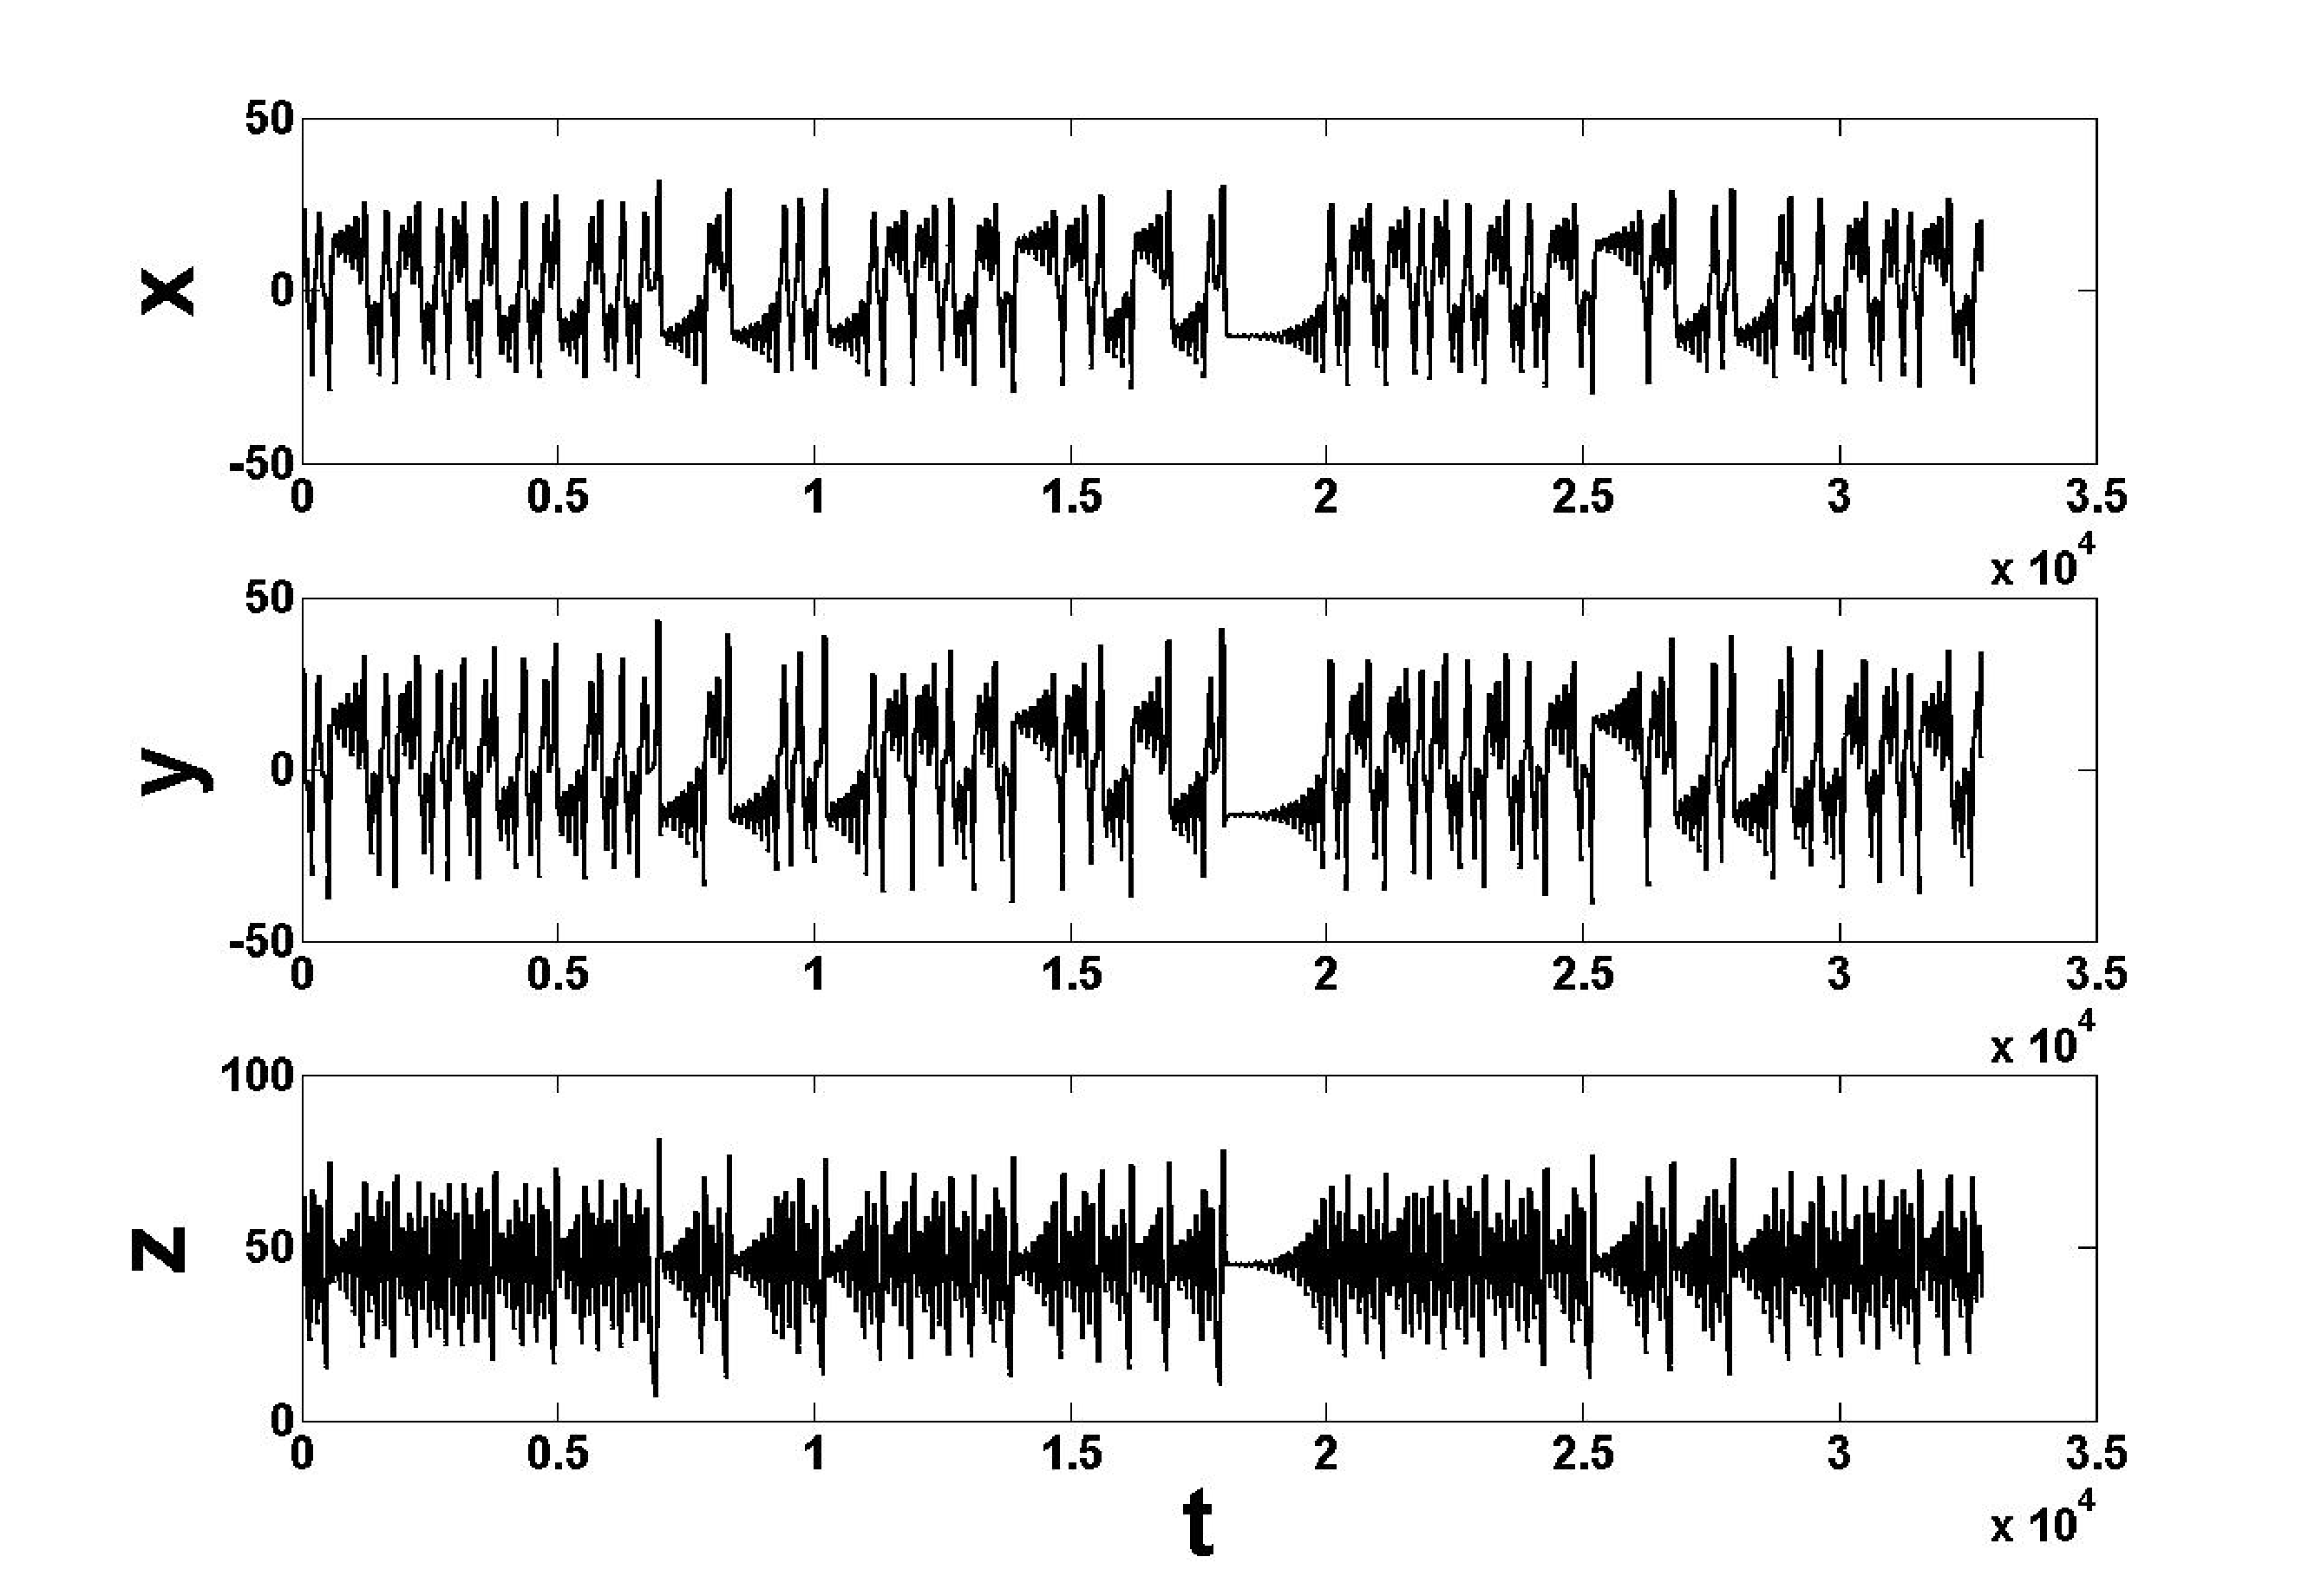
\includegraphics[width=1\columnwidth]{LorenzTiempo.pdf}\\
	\caption{Series temporales del atractor de Lorenz.}\label{fig:tiempo}
\end{figure}
%
\begin{figure}
	\centering
	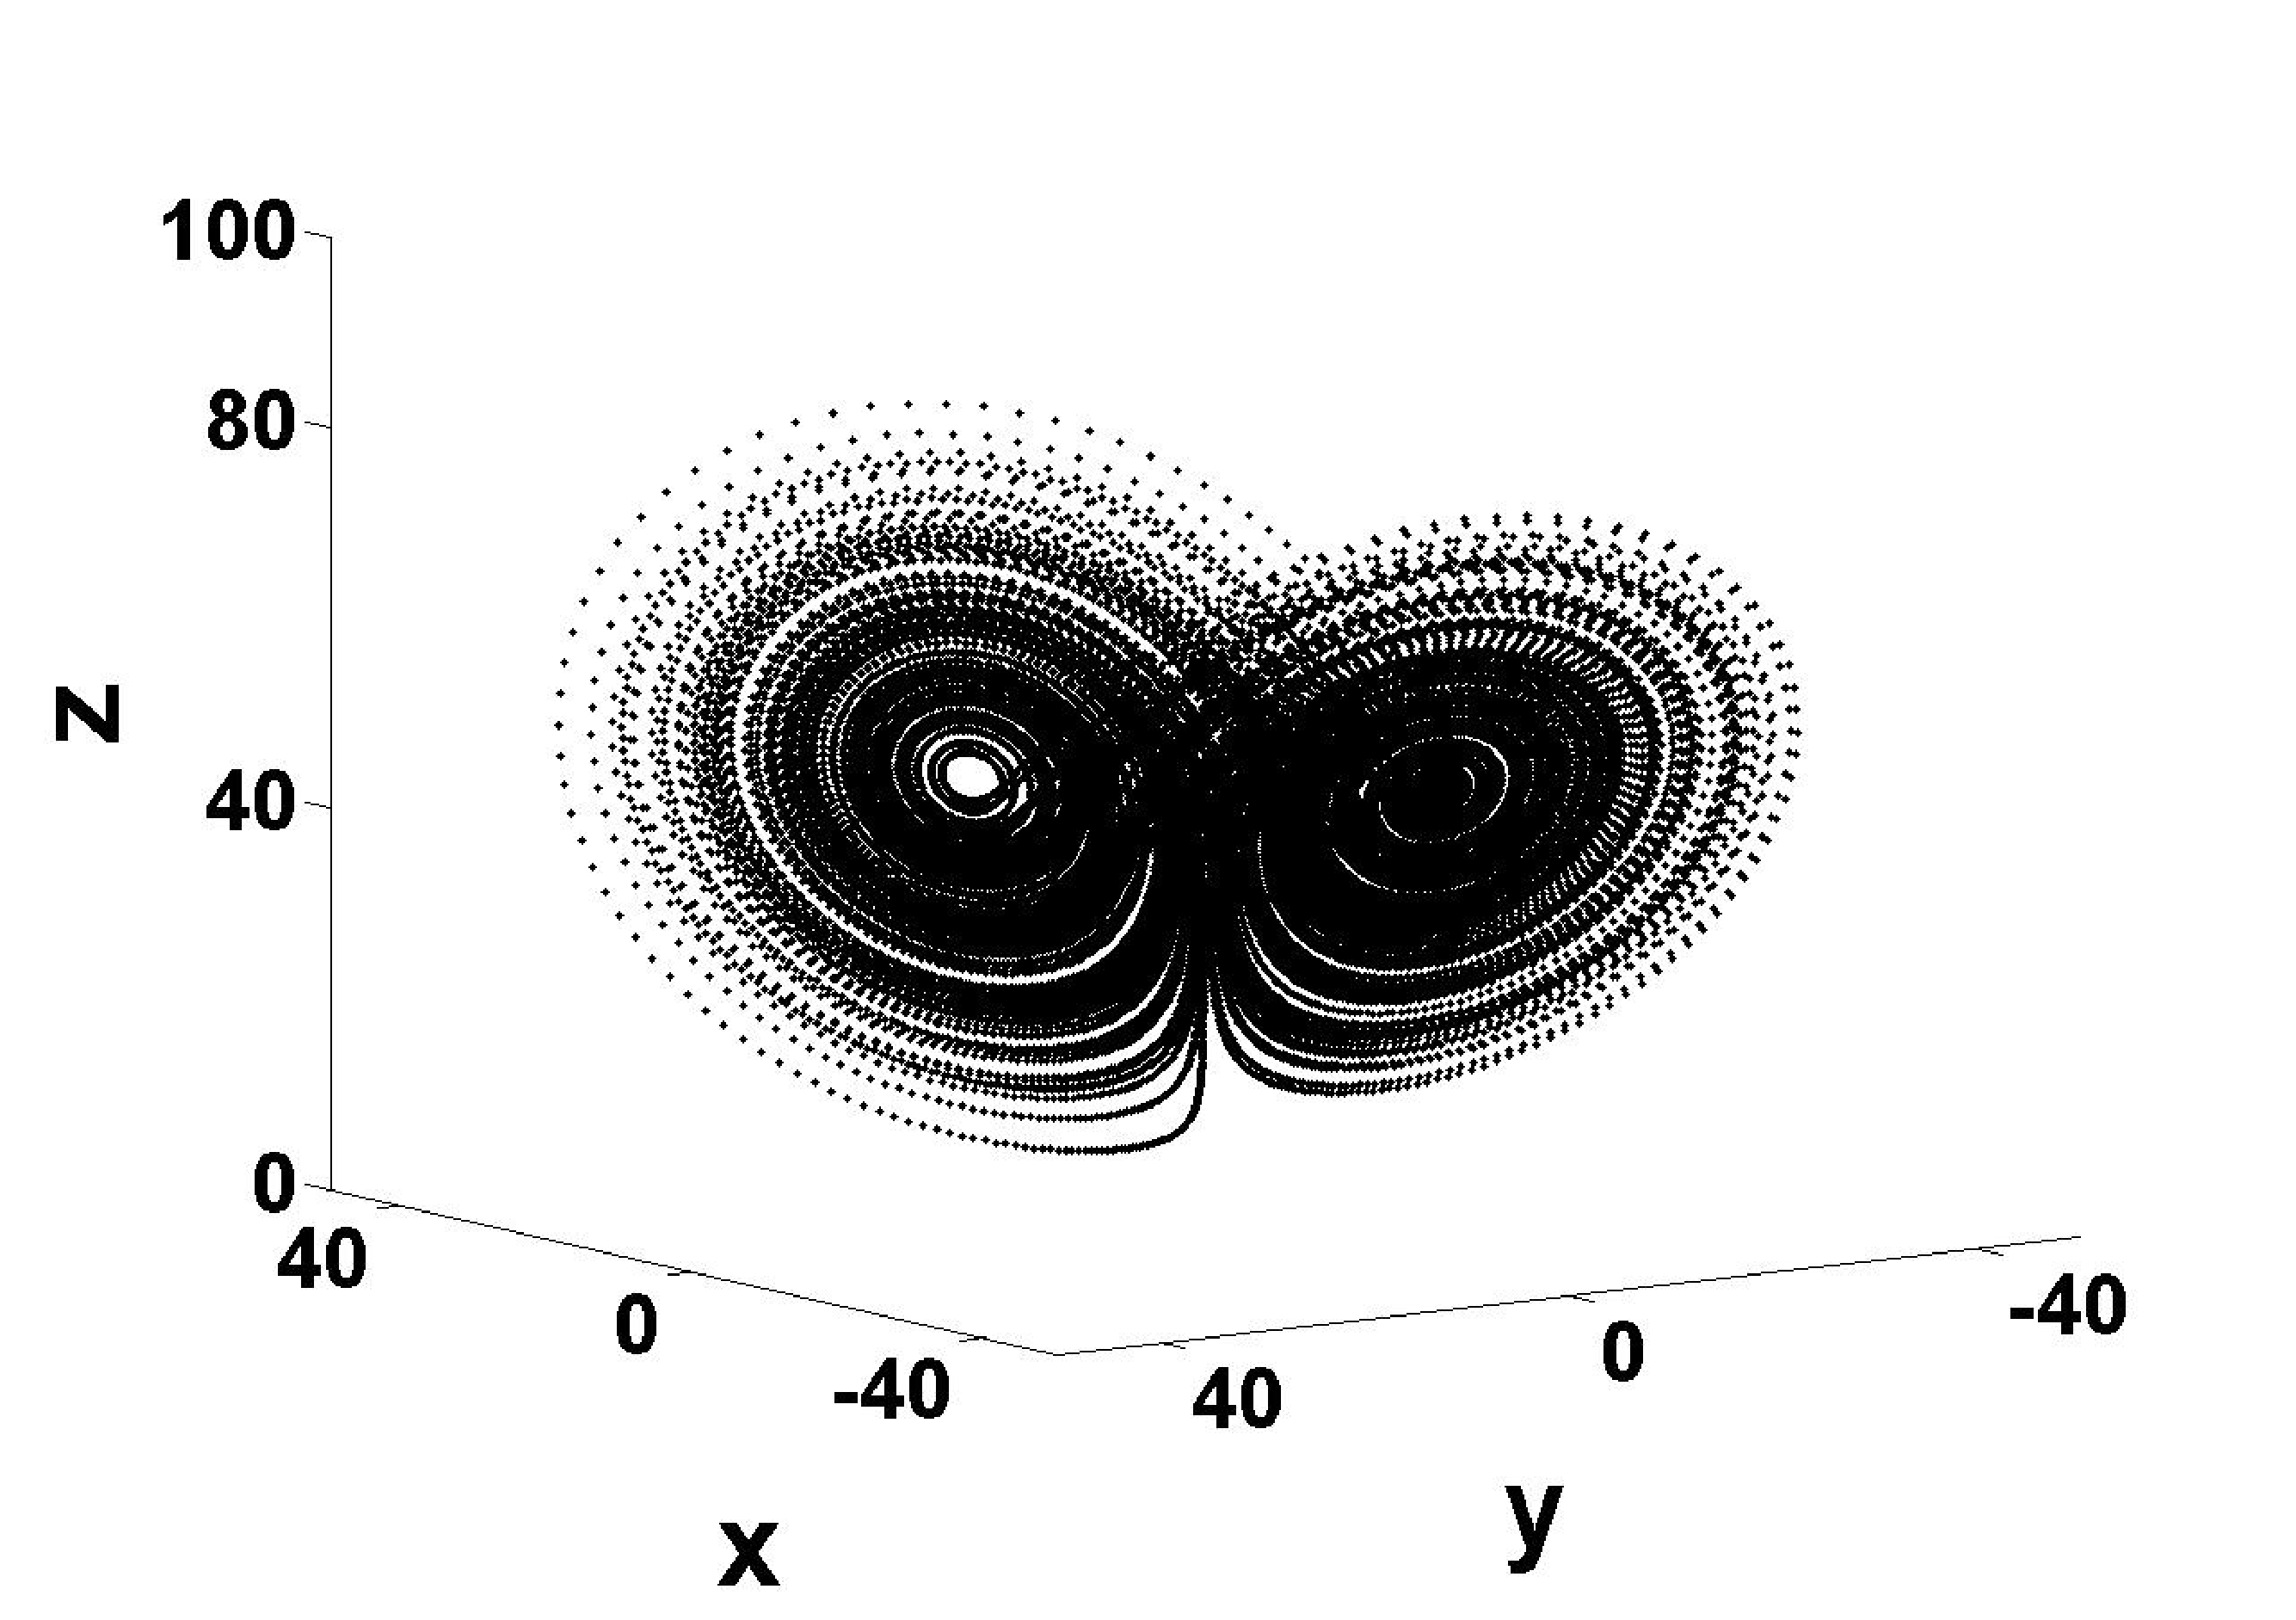
\includegraphics[width=1\columnwidth]{LorenzAtractor}\\
	\caption{Atractor de Lorenz.}\label{fig:atractor}
\end{figure}

El hardware requerido se muestra en el Cuadro \ref{tabla:TablaImpLorenz1}. Allí se muestra una comparación entre los resultados de la compilación en las tres representaciones numéricas estudiadas:
\begin{itemize}
\item \textit{aritmética de punto flotante}: los dos casos, precisión simple y doble (Flotante($32$bits) y Flotante($64$bits) respectivamente),
\item \textit{aritmética entera} (Enteros($54$bits)) y
\item \textit{aritmética de punto fijo}: los dos casos, ambos con $9$ bits de parte entera más $1$ bit de signo más los bits para la parte decimal, $22$ bits para punto fijo ($32$bits) o $54$ bits para punto fijo ($64$bits) respectivamente.
\end{itemize}
%
\begin{table*} [tb]
\begin{center}
\caption{Resultados de compilación en CYCLONE III EP3C120F780C7.}
\label{tabla:TablaImpLorenz1}
\begin{tabular}{c|c|c|c|c|c|c|}
	\cline{2-6}
	& \begin{tabular}[c]{@{}c@{}} Punto fijo\\($32$bits)\end{tabular} & \begin{tabular}[c]{@{}c@{}} Punto fijo\\($64$bits) \end{tabular} & \begin{tabular}[c]{@{}c@{}} Flotante\\($32$bits) \end{tabular} & \begin{tabular}[c]{@{}c@{}} Flotante\\($64$bits) \end{tabular} & \begin{tabular}[c]{@{}c@{}} Enteros\\($54$bits) \end{tabular} \\ \hhline{~=====} \cline{1-1}
\multicolumn{1}{|c|}{Elementos lógicos [Total]}     &       $2392$        &       $6104$        &      $8176$       &      $17532$      &      $1297$ \\ \hline
\multicolumn{1}{|c|}{Elementos lógicos [\%]} 		&        $2.00$        &        $5.12$        &       $6.86$       &      $14.72$       &      $1.08$ \\ \hline
\multicolumn{1}{|c|}{Total de registros}          	&       $1658$        &       $1754$        &      $4753$       &      $8532 $      &       $159$ \\ \hline\hline
\multicolumn{1}{|c|}{Reloj $f_{max}$ [MHz]}         &       $37.82$        &       $20.51$        &       $7.48$       &       $5.42$       &      $55.38$ \\ \hline
\multicolumn{1}{|c|}{Throughput [Mbs]}           	&      $1210.24$      &       $656.32$       &      $14.96$       &      $173.44$      &    $1772.16$ \\ \hline
\end{tabular}
\end{center}
\end{table*}

La implementación aritmética de enteros es la que emplea recursos mínimos y admite un $f_{max}$ más alto, la razón de esto es que las ecuaciones implementadas fueron optimizadas previamente para esta aplicación en particular.
En el caso de la representación de punto flotante, la optimización se realizó para disminuir el área, pero se pueden aplicar otras técnicas de optimización para mejorar la frecuencia o el consumo de energía \cite{Giri2012, Gokul2004}.

Para utilizar este sistema como PRNG, los datos de salida se procesan con las técnicas \textit{descarte} y \textit{concatenado}.
Ambas técnicas mantienen los bits menos significativos porque presentan el comportamiento más variable.
En el caso de la técnica de \textit{concatenado}, la parte más ruidosa de cada variable de estado se mantiene y se recombina, y se obtiene una salida de secuencia de $32$-bits en cada iteración.

Se generaron archivos de datos de análisis estocástico con $3~000~000$ palabras de $32$-bits cada uno, para $\Delta t = 2^{-n}$, con $n = 6$, $7$, $8$, $9$ y $10$.
Se calcularon las pruebas DIEHARD para todos los archivos generados.
En el Cuadro \ref{tabla:TablaImpLorenz2} se informan algunos de los resultados más relevantes.
\begin{table*} [tb]
\begin{center}
\caption{Resultados del test DIEHARD. $\Delta t = 2^{-n}$.}
\label{tabla:TablaImpLorenz2}
\begin{tabular}{c|c|c|c|c|c|c|}
	\cline{2-7}
	                        & $n$ & 6 & 7 & 8 & 9 & 10 \\ \hhline{~======}\cline{1-1}
	\multicolumn{1}{|c|}{\multirow{2}{*}{\begin{tabular}[c]{@{}c@{}}\\ Flotante\\ ($64$ bits)\end{tabular}}} &    $x_{disc}$    &    no    &    no     &     si     &     si      &      no      \\ \cline{2-7}
	\multicolumn{1}{|c|}{}                         &    $y_{disc}$    &    no    &    no     &     si     &     si      &      no      \\ \cline{2-7}
	\multicolumn{1}{|c|}{}                         &    $z_{disc}$    &    si    &    si     &     si     &     no      &      no      \\ \cline{2-7}
	\multicolumn{1}{|c|}{}                         &      $zyx$       &    no    &    no     &     no     &     no      &      si      \\ \hline\hline
	\multicolumn{1}{|c|}{\multirow{2}{*}{\begin{tabular}[c]{@{}c@{}}\\ Punto fijo\\ ($64$ bits)\end{tabular}}} &    $x_{disc}$    &    si    &    si     &     no     &     no      &      no      \\ \cline{2-7}
	\multicolumn{1}{|c|}{}                         &    $y_{disc}$    &    si    &    si     &     no     &     no      &      no      \\ \cline{2-7}
	\multicolumn{1}{|c|}{}                         &    $z_{disc}$    &    si    &    si     &     no     &     no      &      no      \\ \cline{2-7}
	\multicolumn{1}{|c|}{}                         &      $zyx$       &    si    &    si     &     si     &     no      &      no      \\ \hline\hline
	\multicolumn{1}{|c|}{\multirow{2}{*}{\begin{tabular}[c]{@{}c@{}}\\ Enteros\\ ($54$ bits)\end{tabular}}} &    $x_{disc}$    &    si    &    si     &     no     &     no      &      no      \\ \cline{2-7}
	\multicolumn{1}{|c|}{}                         &    $y_{disc}$    &    si    &    si     &     no     &     no      &      no      \\ \cline{2-7}
	\multicolumn{1}{|c|}{}                         &    $z_{disc}$    &    si    &    si     &     no     &     no      &      no      \\ \cline{2-7}
	\multicolumn{1}{|c|}{}                         &      $zyx$       &    si    &    si     &     si     &     si      &      si      \\ \hline
\end{tabular}
\end{center}
\end{table*}

Este Cuadro muestra que en los casos de implementaciones de enteros y punto fijo la técnica de aleatorización de \textit{descarte} funciona mejor a medida que $\Delta t$ aumenta porque, para elementos $\Delta t$ menores, las series temporales son más correlacionadas y esta técnica de aleatorización no los mezcla lo suficiente.
Para utilizar valores de $\Delta t$ más bajos, más bits deben descartarse para obtener buenos PRNG.
Por otro lado, la técnica de aleatorización de \textit{concatenación} funciona bien independientemente del valor de $\Delta t$ (dentro del rango analizado).